\documentclass[tikz,border=2pt]{standalone}
\usepgflibrary{arrows}
\definecolor{lightblack}{RGB}{74,74,74}
%\input{C:/Users/cagne/Desktop/Alberto/Templates/macro/packages}
\usepackage{pgfplots,relsize}
\usepgfplotslibrary{fillbetween}
\usetikzlibrary{shapes,calc,arrows,through,
intersections, decorations,patterns,hobby}
\usetikzlibrary{decorations.markings, bending,arrows.meta,calc}

\usepackage{amssymb}
\usepackage{amsmath}
%\usepackage{amsthm}
\usepackage{amsfonts}
\usepackage{amscd}

\begin{document}

\pgfplotsset{
scale only axis,
width=8.7cm,
unit vector ratio*=1 1 1,
every axis/.append style = {
font=\relsize{0},
% riguarda le tick labels
%line width = 1.2pt,
% oppure: thin, semithick, thick,
% very thick
%tick style = {line width = 1.2pt}
},
compat=1.3,
  tick label style={font=\scriptsize},
  %label style={font=\small},
  legend style={font=\normalsize},
%every axis x label/.append style = {
%font = \relsize{1}
%},
%every axis y label/.append style = {
%font = \relsize{-1},
%rotate = -90,
%xshift = 17pt
%yshift = -1.4em
%},
major grid style = {
line width = 0.8pt,
gray, opacity=0.5
%dash pattern = on 8pt off 4pt
},
%every axis title/.append style = {
%font = \relsize{1}
%}
disabledatascaling
}



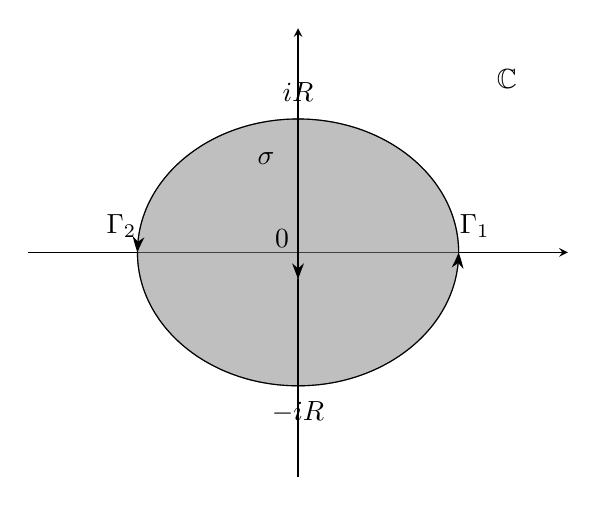
\begin{tikzpicture}
\begin{axis}[axis lines=middle,
            %xlabel=$x$,
            %ylabel=$y$,
            ymax=1.4,
            ymin=-1.4,
            xmax=1.4,
            xmin=-1.4,
            %axis x line=middle,  
            %axis y line=left,
            enlargelimits,
            xtick=\empty, %={1.15,1.4},
            ytick=\empty,%{0.8,1.2},
            %xticklabels={$x_1$,$x_2$},
            %yticklabels={$y_1$,$y_2$}
            ,clip=false]
\def\yone{0.8}
\def\ytwo{1.2}
\def\xone{1.1}
\def\xtwo{1.4}
%\def\r{1.4}

\draw[fill=gray, opacity=0.5] (0,0) circle (1);

\node[] at (axis cs: 1.3,1.3){$\mathbb{C}$};

\node[] at (axis cs: -0.2,0.7){$\sigma$};

\node[] at (axis cs: -0.1,0.1){$0$};

\node[] at (axis cs: 1.1,0.2){$\Gamma_{1}$};

\node[] at (axis cs: -1.1,0.2){$\Gamma_{2}$};

\node[] at (axis cs: 0,1.2){$iR$};

\node[] at (axis cs: 0,-1.2){$-iR$};



\draw[-{Stealth[length=0.2cm,bend]}]  (0,-1) arc (-90:0:1);

\draw (1,0) arc (0:90:1);

\draw[-{Stealth[length=0.2cm,bend]}]  (0,1) arc (90:180:1);

\draw (-1,0) arc (180:270:1);

\draw[-{Stealth[length=0.2cm,bend]}]  (0,1)--(0,-0.2);

\draw  (0,-0.2)--(0,-1);

        
%\draw[decoration={markings, mark=at position 0.5 with {\arrow{>}}}, postaction={decorate}]
%        (0,1) arc (90:270:1);
%        
%\draw[decoration={markings, mark=at position 0.25 with {\arrow{>}}, mark=at position 0.75 with {\arrow{>}}}, postaction={decorate}]
%        (0,1)--(0,-1);

%%
%\draw[pattern=north west lines, pattern color=gray!50, rounded corners=2pt] (axis cs: 1,0.2) to[out=60,in=-70] (axis cs: 1.5,1) to[out=100,in=-100] (axis cs: 1.3,1.7) to[out=70,in=0] (axis cs: 0.7,1.9) to[out=200,in=100] (axis cs: 0.5,0.9) to[out=-90,in=60] (axis cs: 0.2,0.05) to[out=-135,in=135] (axis cs: 0.3,-0.5) to[out=30,in=-100] (axis cs: 1.7,-0.2) to[out=160,in=-120] (axis cs: 1,0.2) ;
%
%
%%%%%%%%%%%%%%%%%%%%%%%%%%%%
%
%\begin{scope}
%\clip (axis cs: 1,0.2) to[out=60,in=-70] (axis cs: 1.5,1) to[out=100,in=-100] (axis cs: 1.3,1.7) to[out=70,in=0] (axis cs: 0.7,1.9) to[out=200,in=100] (axis cs: 0.5,0.9) to[out=-90,in=60] (axis cs: 0.2,0.05) to[out=-135,in=135] (axis cs: 0.3,-0.5) to[out=30,in=-100] (axis cs: 1.7,-0.2) to[out=160,in=-120] (axis cs: 1,0.2) ;
%\fill[blue, opacity=0.6] (axis cs: 0,\yone) rectangle (axis cs: 2,\ytwo);
%\end{scope}
%
%\begin{scope}
%\clip (axis cs: 1,0.2) to[out=60,in=-70] (axis cs: 1.5,1) to[out=100,in=-100] (axis cs: 1.3,1.7) to[out=70,in=0] (axis cs: 0.7,1.9) to[out=200,in=100] (axis cs: -1,0.9) to[out=-90,in=60] (axis cs: 0,0.05) to[out=-135,in=135] (axis cs: 0.3,-0.5) to[out=30,in=-100] (axis cs: 1.7,-0.2) to[out=160,in=-120] (axis cs: 1,0.2) ;
%\draw[thick, densely dashed] (axis cs: 0,\yone) --(axis cs: 2,\yone);
%\draw[thick, densely dashed] (axis cs: 0,\ytwo) --(axis cs: 2,\ytwo);
%\end{scope}
%
%\draw[color=lightblack,->] (axis cs: 0.4,{(\yone+\ytwo)/2}) -- (axis cs: 0.1,{(\yone+\ytwo)/2});
%
%\draw[color=lightblack,->] (axis cs: 1.2,2.02) -- (axis cs: 0.5,2.02);
%\node[above] at (axis cs: 0.9,2.02){$\pi_{2}$};
%
%
%\draw[color=blue,thick] (axis cs: 0,0.8)--(axis cs: 0,1.2);
%
%
%\draw[color=blue,->] (axis cs: -0.3,1.5) to[out=-120,in=150] (axis cs: -0.1,{(\yone+\ytwo)/2});
%\node[above,color=blue] at (axis cs: -0.3,1.5){$\mu_{2}$};
%
%
%%%%%%%%%%%%%%%%%%%%%%%%%%%%%%
%%%% green part for x axis 
%
%\begin{scope}
%\clip (axis cs: 1,0.2) to[out=60,in=-70] (axis cs: 1.5,1) to[out=100,in=-100] (axis cs: 1.3,1.7) to[out=70,in=0] (axis cs: 0.7,1.9) to[out=200,in=100] (axis cs: 0.5,0.9) to[out=-90,in=60] (axis cs: 0.2,0.05) to[out=-135,in=135] (axis cs: 0.3,-0.5) to[out=30,in=-100] (axis cs: 1.7,-0.2) to[out=160,in=-120] (axis cs: 1,0.2) ;
%\fill[green, opacity=0.6] (axis cs: \xone,-1) rectangle (axis cs: \xtwo,2);
%\end{scope}
%
%
%
%\begin{scope}
%\clip (axis cs: 1.5,0.2) to[out=60,in=-70] (axis cs: 1.5,1) to[out=100,in=-100] (axis cs: 1.3,1.7) to[out=70,in=0] (axis cs: 0.7,1.9) to[out=200,in=100] (axis cs: 0.5,0.9) to[out=-90,in=60] (axis cs: 0.2,0.05) to[out=-135,in=135] (axis cs: 0.3,-0.5) to[out=30,in=-100] (axis cs: 1.7,-0.2) to[out=160,in=-120] (axis cs: 1.6,0.2) ;
%\draw[thick, densely dashed] (axis cs: \xone,2) --(axis cs: \xone,-1);
%\draw[thick, densely dashed] (axis cs: \xtwo,2) --(axis cs: \xtwo,-1);
%\end{scope}
%
%\draw[color=lightblack,->] (axis cs: {(\xone+\xtwo)/2},0.6) -- (axis cs: {(\xone+\xtwo)/2},0.3);
%
%\draw[color=lightblack,->] (axis cs: {(\xone+\xtwo)/2},-0.25) -- (axis cs: {(\xone+\xtwo)/2},-0.05);
%
%\draw[color=lightblack,->] (axis cs: 2,1.7) -- (axis cs: 2,1.3);
%\node[right] at (axis cs: 2,1.5){$\pi_{1}$};
%
%
%\draw[color=green,thick] (axis cs: \xone,0)--(axis cs: \xtwo,0);
%
%
%%%%%%%%%% green arrow
%\draw[color=green,->] (axis cs: 2,0.7) to[out=-60,in=80] (axis cs: {(\xone+\xtwo)/2+0.05},0.07);
%\node[above,color=green] at (axis cs: 2,0.7){$\mu_{1}$};
%
%
%%%%%% two x
%\node[above right,xshift=-2.6pt, yshift=-2pt] at(axis  cs:\xone,0){{\scriptsize $x_{1}$}};
%\node[above right,xshift=-2.6pt, yshift=-2pt] at(axis  cs:\xtwo,0){{\scriptsize $x_{2}$}};



\end{axis}
\end{tikzpicture}


\end{document}